\section{Controlling a Smart Home}
\label{sec:introduction:gesture-control}
% \todo[author=Kasper]{Vi bør nok lige komme på en bedre titel til dette afsnit.}

Controlling a smart home is a matter of changing the state of smart devices in the home. For example, opening or closing a window, locking or unlocking the door or changing the tempreature on the thermostat. There are a variety of ways to control a smart home including, but not limited to, the following.

\begin{itemize}
\item Using a smartphone application.
\item Using a physical remote control such as the Logitech Harmony Remote\footnote{http://www.logitech.com/harmony-remotes}.
\item Using rules that are automatically triggered when specific events occur, e.g. the time of the day changes.
\end{itemize}

An alternative way of controlling a smart home is using motion gestures using a wearable worn by the user. In the survery \cite{Kela2006}, 76\% of 37 people found that gestures was a natural way of controlling devices, 8\% found it unnatural and the remaining 16\% left the question unanswered.

In this report we wish to investigate the option of controlling a smart home using motion gestures recognized using a wearable.

Another project concerned with gesture controls in a smart home is the Reemo\footnote{http://www.getreemo.com}, a wearable targeted towards seniors which enable them to control smart devices by performing motion gestures with a hand. When controlling a device, the user must point at the device as illustrated in \cref{fig:introduction:gesture-control:reemo} and then perform a pre-programmed gesture which maps to an action on the targeted smart device. Upon installation of the system, receivers are placed nearby the smart devices the user desires to control. The user points at this receiver when controlling a device, thus limiting the devices which a user can control to those within line of sight.

\begin{figure}
\centering
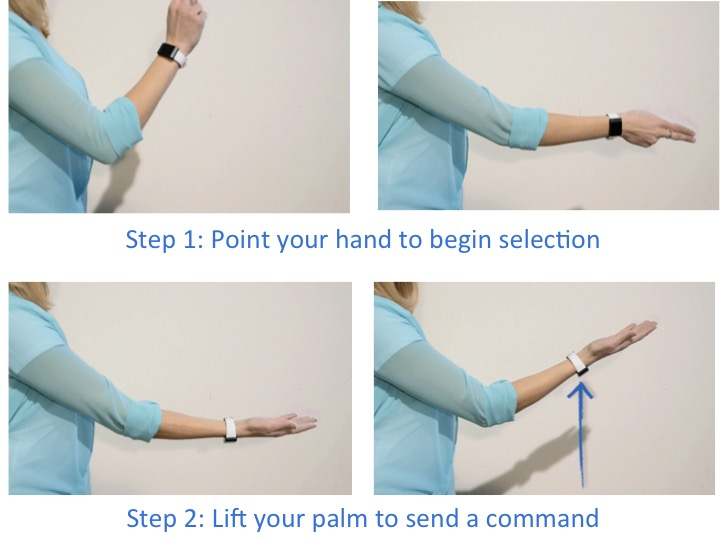
\includegraphics[width=0.65\textwidth]{images/reemo}
\label{fig:introduction:gesture-control:reemo}
\caption{Using the Reemo wearable to control a smart device. Image from \cite{prespecialisation}.}
\end{figure}

Reemo has not published any details about how their technology works.

\subsection{Required Amount of Gestures}

The amount of gestures a person is able to recall is limited and the smaller a set of gestures is, the easier it is for a person to remember. This is supported by \cite{Kela2006} wherein a user study reported that users would like to be able to use the same gesture for multiple devices, as well as keep the set of gestures available should be kept relatively small.
The ideal size of a gesture set is unknown, in part because people have differing recollection capabilities. Miller \cite{miller1956magical} theorized that an adult can store $7 \pm 2$ objects in their working memory.
Reuse of gestures across multiple devices results in fewer gestures overall that a person has to remember, but imposes the challenge of making sure that only the user's intended target device reacts to a gesture.

The scenario presented in \cref{sec:analysis:scenarios} has a total of 30 actions that can be triggered. If we assume there is only one music centre in the apartment that can be controlled from multiple rooms, we can reduce the amount of actions to 24.

If we make a system in which one gesture maps to a single action, a minimum of 24 gestures would be required to control the smart home shown in \cref{fig:analysis:scenario:apartment}. Based in on \cite{Kela2006,miller1956magical} it is our belief, that a user cannot remember 24 gestures and more so, cannot remember which action each of the gestures trigger.

By taking the \emph{context} in which the user is situated into account, we can reduce the number of gestures a user must remember in order to control the smart home. \emph{Context} is defined and discussed in \cref{sec:analysis:context}. Examples of information that contribute to knowledge about the context a user is situated in, includes the position of the user, e.g. which room he is in.

From the scenario presented in \cref{sec:analysis:scenarios} it is apparent, that in a gesture controlled system in which the performance of a gesture triggers different actions depending on the room a user is in, the maximum amount of gestures a user must remember equals the number of actions that can be triggered in the room with the most actions.

In the scenario, the living room has a total of eight different actions, making in the room with most actions. Therefore a total of eight different gestures are required in the system.

%%% Local Variables:
%%% mode: latex
%%% TeX-master: "../../master"
%%% End:
